\subsection{Fault Analysis }

We  compare the impact of losing $d$ machines 
to the the VC and VO approaches.  
The replication degree of the backup storage 
is $r$ for regular content blocks and $r=3$ is a typical setting in the distributed
file system~\cite{Hadoop,GFS}.
in The VC approach, a special replica degree $r_c$ used for CDS blocks where $r_c>r$. 
Noted that the storage cost for VO with full deduplication is $b_u *r$
while it is
\[ r*b*\delta(1 -   (\frac{k}{b_u})^{1-\alpha}) +k*(r-r_c).
\]

For each rank $i$ block which appears $C_i$ times  among $V$ virtual machines.
Assigning this block to virtual machines can be viewed as a classical ball-bin assignment
approximated by a Poisson distribution. Namely the virtual machines that share this block
is approximated as $1 -  e^{C_i/V}$.
Thus the average number of VMs that share a block is:
\[
(1-\delta) + \delta \sum_1^{u_b} \frac{1 -  e^{C_i/V}}{u_b}.
\]
Any failure of a block would impact the above number of virtual machines.
In VO, the number of VMs that share a block is:
\[
\sum_1^{u_b'} \frac{1 -  e^{C_i'/V}}{u_b'}.
\]

Next we discuss how a failure of $d$ machines impacts the VM snapshots in VC.
When $d<r$, there is no loss of data in the snapshot storage.
When $r_c> d \ge r$, some of data blocks in the storage are lost, and we compute the number of VMs that could
suffer the loss of their snapshots.
When $d \ge r_c$, some of CDS blocks are affected.
In VC, the blocks in CDS are stored in a container manner (superblock), and they are shared by many VMs.
The number of data containers stored with replication degree $r$ for
referenced by each VM is:
\[
N_1= \frac{b}{v*s} (1-\delta) +b/(v*s)\delta (1 -  (\frac{k}{b_u})^{1-\alpha})
\]
The number of CDS data containers stored with replication degree $r_c$ for
referenced by each VM is:
\[
N_2= \frac{b}{v*s}\delta (\frac{k}{b_u})^{1-\alpha}.
\]



%Thus the number of VMs using a block =    $(1-s_c)  + s_c *L$.

When there are $r \le d<r_c$ machines failed and the probability of
a container failure depends on if all replicas of this container reside in the failed machines.
\begin{multline}
Probability (\mbox{ a VM fails in VC})\\
= 1- Probability (\mbox{ a VM has no data container loss}) \\
= 1-  Probability(\mbox{ A container has no data loss})^{N_1}
%\end{split}
\end{multline}

%Probablity(\mbox { no loss for this  block}) = 1 - Probability (\mbox{ this block in d failed machiens})
\begin{multline}
%\begin{split}
Probability(\mbox{A container no data loss})\\
= 1- Probability (\mbox{ this container is in d failed machines})\\
=  1- \frac{\binom{d}{r}} { \binom{p}{r} }.
%\end{split}
\end{multline}

When $r_c \leq d$, the CDS data containers in VC can also have a loss. 
\begin{multline}
Probability (\mbox{ a VM fails in VC})\\
= 1-  Probability(\mbox{ A container has no data loss})^{N_1}* \\
Probability(\mbox{ A CDS container has no data loss})^{N_2}\\
= 1 - 
(\frac{ \binom{d}{r}} { \binom{p}{r} })^{N_1} 
*
(\frac{ \binom{d}{r_c}} { \binom{p}{r_c} })^{N_2} 
%\end{split}
\end{multline}

By comparison, the probability that a VM has data loss is close to
1 once  there are  $d \ge r$ failed machines. That is because there are more data blocks
shared among VMs. Any failure of these blocks causes many more VMs to fail.

The rate of increase in node failures can be seen in Figure~\ref{fig-vm-failure}
(for a 100 node cluster).
The graph assumes 10X40GB snapshots per VM with 18\% unique data after local
dedup and 64MB filesytem chunks (which results in 1792 filesystem chunks per
VM). We assume 18\% unique data after local dedup because that is what our
snapshots have shown.

\begin{figure}[ht]
  \centering
  %\includegraphics[scale=.45,natwidth=511,natheight=276]{vo_links}
	\begin{tikzpicture}
		\begin{axis}[
		%title={Node failure affect on VMs},
		xlabel={Number of nodes failed},
		ylabel={chance that a VM is affected (\%)},
		%extra y ticks={4.5,5.5,6.5} %because it only shows 4,5,6,7
		]
		\addplot[color=blue,mark=*] table{figures/vm_failure.txt};
		\end{axis}
	\end{tikzpicture}
  \caption{Percent chance that a VM is affected as storage nodes fail}
  \label{fig-vm-failure}
\end{figure}

\comments{
We use the following parameters  during the analysis
\begin{itemize}
\item 	$V$ is the number of VMs. $m$ is the number of physical machines hosting the backup storage.
$d$ is the number of machines failed.
\item In the VC approach, $s_c$  of them in the backup storage
are shared by others with a zipf distribution. $(1-s_c)$ 
of them  is unique (nobody shares with them).
$L_c$ is the average number of VMs sharing a block (if it is in CDS for the VC approach.
$b_c$ is the number of shared blocks in VC.
\item In the VO approach, $s_o$ is the number of blocks shared.
$L_o$ is the average number of VMs sharing a block. 
\item $b$ is the  number of blocks stored in the storage after deduplication.
 \end{itemize}

The distribution of data blocks shared among VMs in VC follows a zipf distribution.
Given a VM block, the probability of being rank $x$ block is $P(x) = P(1) * x^{-\alpha}$
where $P(1)$ is the probability of being rank 1 most popular block.
Since $\sum P(x)= 1$, $P(1)= \frac{1}{\sum_1^{b_c} x^{-\alpha} }$.
Let $y$ be the number of VMs sharing rank $x$ block in VC, and  then  $y= V* P(x)$.

Thus the average number of VMs sharing a data block in the VC backup storage is:
\begin{equation}
%\begin{align}
\begin{split}
L_c& =  (1-s_c)*1 + s_c \sum_1^{b_c} P(x) * y \\
& =  (1-s_c)*1 + s_c \sum P(1)^2 *  x^{-2\alpha} *  V.
\end{split}
%\end{align}
\end{equation}

We can build a bipartite graph representing the association from unique data blocks
to their corresponding VMs. An association edge is  drawn  from a data block  to a VM 
if this block is used by this VM, 
The average incoming degree of VM nodes is equal to
the average outgoing degree of data blocks, which is $L_c$. 


\begin{figure}[htbp]
\centering
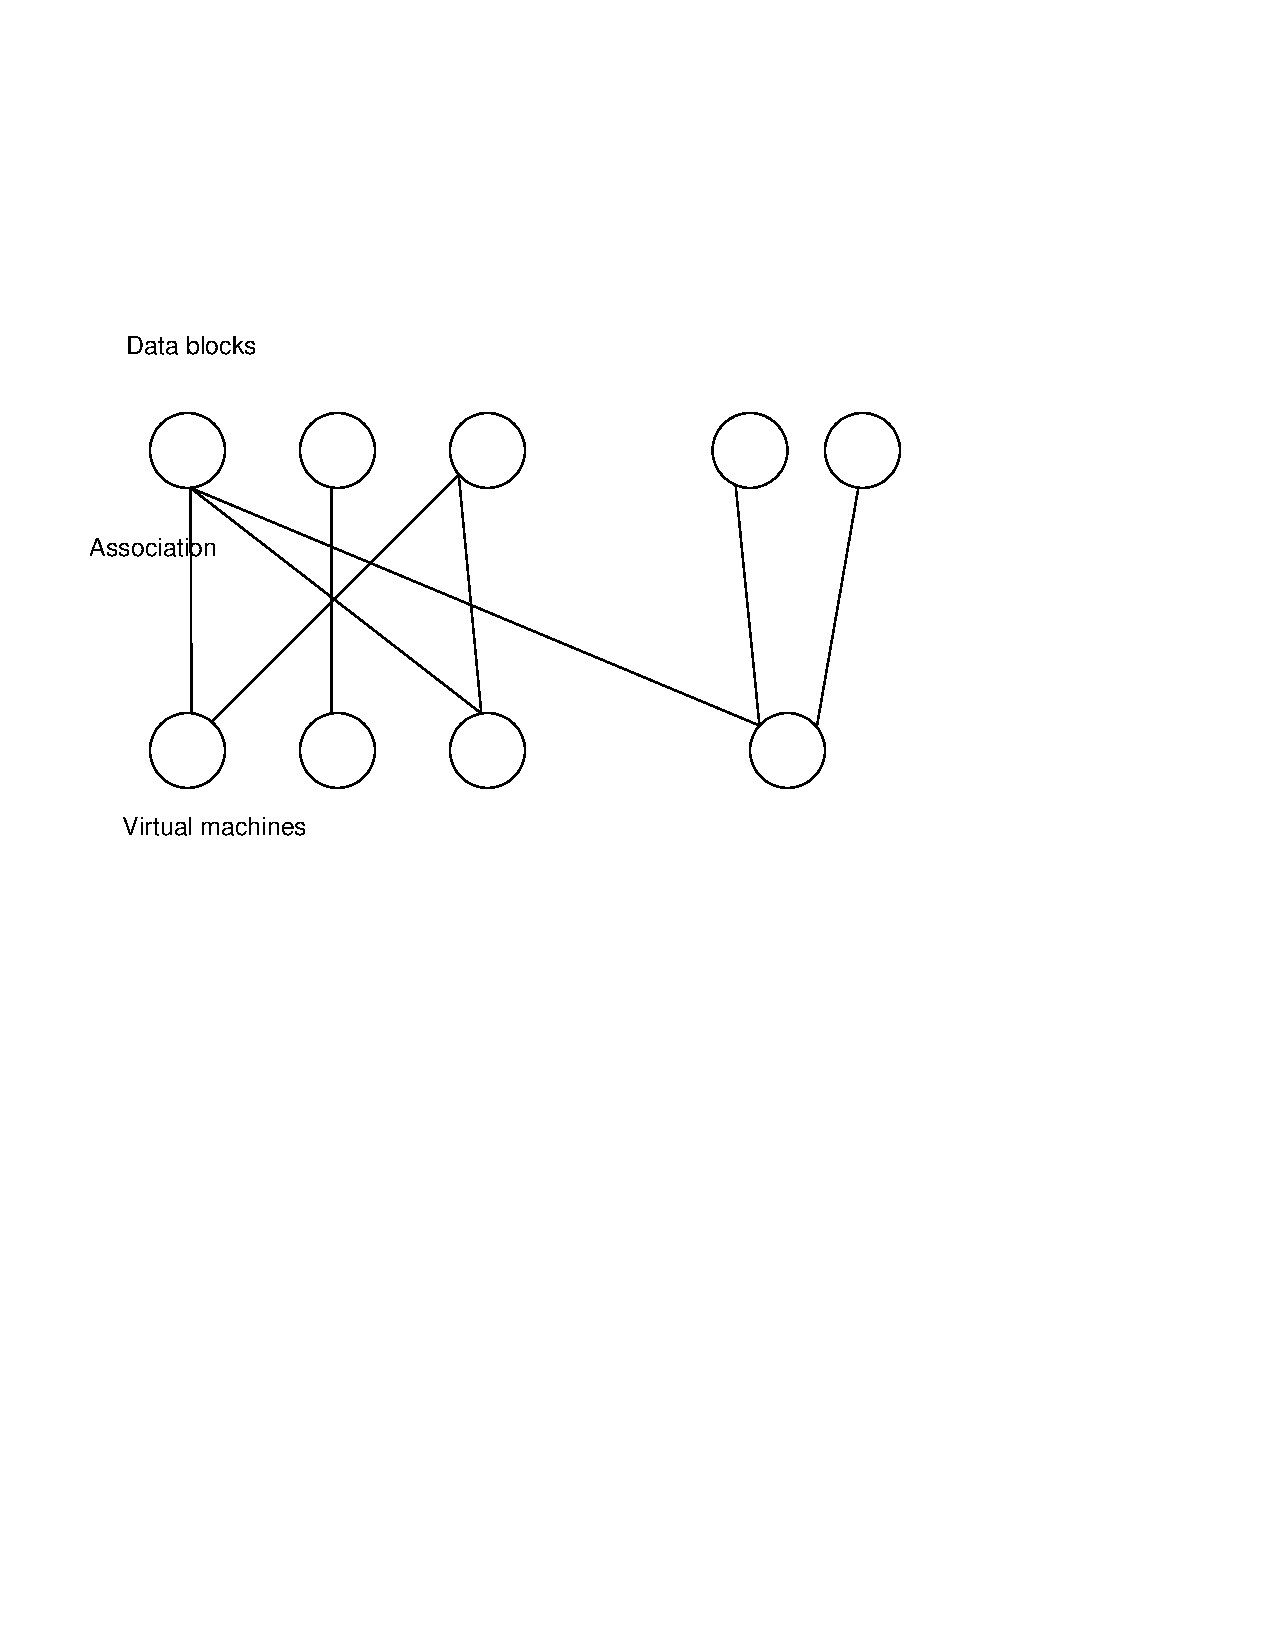
\includegraphics[width=0.45\textwidth]{shared.pdf}
\caption{Assoication of data blocks to VMs.}
\label{fig:shared}
\end{figure}


Under $d$ failed machines, the  expected number of VMs 
which suffer from data loss in VC is
\begin{multline}
%\begin{split}
 \sum_{1}^{V}  ( Probability (\mbox{ a VM fails)}) \\
= \sum_{1}^{V}  ( 1- Probability (\mbox{ a VM has no data loss)}) \\
= V ( 1-  Probability(\mbox{ A block has no data loss} )^{L_c} ).
%\end{split}
\end{multline}

%Thus the number of VMs using a block =    $(1-s_c)  + s_c *L$.

When there are $d$ machines failed and the probability of
a block failure depends on if all replicas of this block reside in the failed machines.
When $r< d <r_c$,  only unshared data blocks can fail in VC. Then
%Probablity(\mbox { no loss for this  block}) = 1 - Probability (\mbox{ this block in d failed machiens})
\begin{multline}
%\begin{split}
Probability(\mbox{ A block has data loss})\\
= (1-s_c) (1- Probability (\mbox{ this block in d failed machines}))\\
= (1-s_c) (1- \frac{ \binom{d}{r}} { \binom{m}{r} }).
%\end{split}
\end{multline}
When $r_c \leq d$, shared data blocks in VC can have a loss. 
\[
Probability(\mbox{A block has data loss})
= 
(1-s_c) (1- \frac{ \binom{d}{r}} { \binom{m}{r} })
+ s_c (1- \frac{ \binom{r_c}{d}} { \binom{m}{r_c} }).
\]

By comparison, under $d$ failed machines, the  expected number of VMs 
which suffer from data loss in VO is
\[
V ( 1-  (1- \frac{ \binom{d}{r}} { \binom{m}{r} })^{L_o} ).
\]
where
\[
L_o = (1-s_o) + s_o \sum_1^b  P(1)^2 *  (x')^{-2\alpha'} *V.  
\]

%the above model assumes uniform distribution of blocks and doesn't provide compelling numbers
%with 3 replicas, 100 machines, and only 3 failures the chance of a single 10GB VM surviving is 9.11*10^-8
%if we wanted to include it we probably want a model that includes containers, but that might be too complex
%to be useful.
}

Figure~\ref{fig-vo-links} shows the average number of links to a given block in the global index as more VMs are added. The first 15 VMs are all windows machines, so that explains the initial higher values, but for the most part the average number of links is between 1.5 and 2.


\begin{figure}[ht]
  \centering
  %\includegraphics[scale=.45,natwidth=511,natheight=276]{vo_links}
	\begin{tikzpicture}
		\begin{axis}[
		%title={VO Block links},
		xlabel={Number of VMs added},
		ylabel={Avg. Links to a Block},
		%extra y ticks={4.5,5.5,6.5} %because it only shows 4,5,6,7
		legend pos=south east
		]
		\addplot[color=blue,mark=*] table[x=VMs,y=Measured] {figures/vo_links.txt};
		\addplot[color=red,mark=square*] table[x=VMs,y=Theoretical] {figures/vo_links.txt};
		\legend{Measured,Theoretical};
		\end{axis}
	\end{tikzpicture}
  \caption{Average number of VMs sharing a block in the global index}
  \label{fig-vo-links}
\end{figure}
\comments{
	=  sum _for_all_block(   Probablity (a block fails) *number of VM sharing this block ))
               = Probability(a block fails) * sum_for_all_blocks (numb of VM shared)
	= Probablity (a block fails) *b *aveageLengthVM
	= [ 1-  C(r, k) /C(n,r)] * b* [ 1+ s *V(1-1/ln V)]
  
----------------------------------------------------------------------       

\subsection{Empirical Validation}
%To validate our theoritical model for the probability of data loss, we computed
%the number of snapshots using each block in a global index for the 350 snapshot
%traces. As you can see in Fig.~\ref{??}, The average number of VMs sharing a block
%%TODO: insert figure generated from data/links_no_cds.dat
%increases linearly with the number of snapshots. For 350 snapshots there are an
%average of 13.1 links to a given block in the global index.
To validate our theoretical model for the probability of data loss, we measured
the number of snapshots and VMs sharing data blocks for our 350 snapshot
dataset. As you can see in Fig.~\ref{??}, the average number of snapshots sharing
a block increases linearly with the number of snapshots. For 350 snapshots
there are an average of 13.1 incoming links to a given data block in the global
index. If we look at the number of VMs sharing a data block rather than
snapshots, in the full dataset on average 1.47 VMs point to a data block in the
index.
%What else do we need from the simulation to validate the model?

\subsubsection{CDS and Fault Tolerance}
%all numbers in this paragraph need to be corrected after I re-run the tests
%using the actual cds generator code
As part of our emprirical validation of our model, we also computed the effects
of the CDS on fault tolerance. If we exclude the top 5\% most popular blocks
and set aside those in the CDS, the average number of links to a non-CDS block
%TODO: insert figure generated from data/links_cds.dat and data/links_wo_cds.dat
drops to 10.3 for 350 snapshots. This means that on average, \~3 fewer
snapshots will be affected by a lost data block in the general data store.
The average number of links to a CDS block however, for 350 snapshots, is
65.7. This suggests that a much higher replication factor is warranted for
the CDS, as on average, a CDS block appears in \~20\% of all the snapshots.
These measured numbers are different from our theoritical model due to the fact
that duplicate data blocks are not uniformly distributed across all VMs.
With uniform distribution of duplicates (and a zipf distribution on the number
of duplicates), there should be on average 2.55 incoming VM links to each
block. Since we show the average number of links to be 1.47 in our actual
traces, the duplicates are
more tighly grouped than the uniform model would predict. This supports
the benefits of using a CDS plus more localized deduplication.

The CDS gives a clear boundary for setting different replication factors,
And our tests suggest that by separating the replication factor for the CDS
and non-CDS blocks, greater fault tolerance can be acheived.

----------------------------------------------------------------------

For CDS model, 85% blocks are using the data from the same VM while upto 10% data is for CDS (we actually only use 5% perhaps).  Thus the overall speaking, at most 10% of data are shared.
Thus  for CDS approach,   the # VM failure caused by k machines is at most  [ 1-  C(r, k) /C(n,r)] * b* [ 1+ 0.10 *V(1-1/ln V)].
For original approach,  [ 1-  C(r, k) /C(n,r)] * b* [ 1+ 0.90 *V(1-1/ln V)].
For large V, the reliability improves by 9 times.
}
